\newpage\section*{Worksheet 6, \Course, \Semester} 
\noindent \Sections 3.4, 3.5, 3.6

\subsection*{Exercises}

\begin{enumerate}
    
    \item A moving object has positive velocity for times $t \in [0,2)$, negative velocity for $t \in (2,4]$, and negative acceleration for $t\in[0,4]$. 
    \begin{enumerate}
        \item Sketch a graph that could represent the objects' position for $t \in [0,4]$. Label your axes.  
        \item Give a formula that could represent the objects' position for $t \in [0,4]$.
    \end{enumerate}
    \item The graph below gives the position of a moving object, $s(t)$ as a function of time, $t$. \begin{enumerate} \item Sketch the velocity and the speed of the object on two separate graphs. \item When the speed constant? \item When is the acceleration non-zero? \end{enumerate}
        \begin{center}
    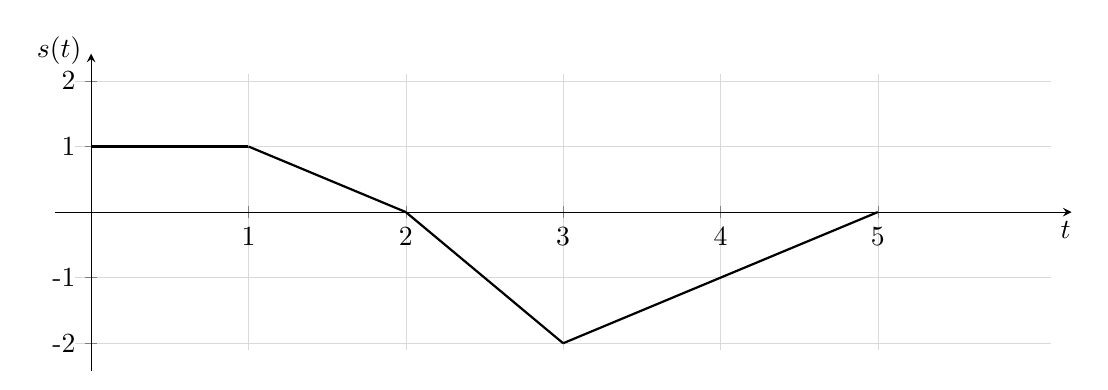
\begin{tikzpicture}[domain=0:6] 
        \begin{axis}[
        width=5.5in,
        height=2in,
        grid=both,
        grid style={line width=.2pt, draw=gray!30},
        clip=false,
        axis lines=middle,
        xmin=-0.1,xmax=6.1,
        ymin=-2.1,ymax=2.1,
        xtick={0,1,2,3,4,5},
        xticklabels={0,1,2,3,4,5},
        ytick={-2,-1,0,1,2},
        yticklabels={-2,-1,0,1,2},
        axis line style={shorten >=-7.5pt, shorten <=-7.5pt},
        xlabel=$t$,
        ylabel=$s(t)$,
        xlabel style={at={(ticklabel* cs:1)},anchor=north west},
        ylabel style={at={(ticklabel* cs:1)},anchor=south east}
        ]
        \addplot[samples=100,domain=0:1,smooth, thick] {1} node[pos=1] (endofplotsquare) {};
        \addplot[samples=100,domain=1:2,smooth, thick] {2-x} node[pos=1] (endofplotsquare) {};
        \addplot[samples=100,domain=2:3,smooth, thick] {4-2*x} node[pos=1] (endofplotsquare) {};        
        \addplot[samples=100,domain=3:5,smooth, thick] {x-5} node[pos=1] (endofplotsquare) {};        
        \end{axis}
    \end{tikzpicture}   
    \end{center}    

    \item \TorF
    \begin{enumerate}
    	\item If $f(x)$ and $g(x)$ are differentiable on the interval $(a,b)$, and $f(x) > g(x)$ over $(a,b)$, then $f'(x) > g'(x)$ on the interval $(a,b)$. 
        \item If $f(x)$ is differentiable for all $x$, and $f(0) = f'(0) = 0$, then $f(x) = 0$ for all $x$. 
        \item If the position of a moving object, $s(t)$, is differentiable for $t\in[0,1]$, and the velocity of the object is positive over $t \in [0,1]$, then the acceleration must also be positive over $t\in[0,1]$. 
    \end{enumerate}    
    
    \item Construct an equation of the tangent line to $y(x)$ at $x= 0$. $$y(x) = \frac{2e^x}{x^2-1}$$
    
	\item Differentiate the following functions. 
    
    \begin{enumerate}
    	\item $y = 1 + f(x^2) g(h(x))$
        \item $y = \frac{3+9\tan x}{\sec x}$
    \end{enumerate}
    
\end{enumerate}